\documentclass[logo,reportComp]{thesis}
\usepackage[cpp,pseudo]{mypackage}
\usepackage{forest}

\usetikzlibrary{automata,backgrounds,fit,shapes,positioning}

\tikzset{->, % makes the edges directed
>=stealth, % makes the arrow heads bold
node distance=2.5cm, % specifies the minimum distance between two nodes. Change if necessary.
every state/.style={thick, fill=gray!10}, % sets the properties for each 'state' node
}

\title{编译原理作业七}
\subtitle{}
\school{数据科学与计算机学院}
\author{陈鸿峥}
\classname{17大数据与人工智能}
\stunum{17341015}
\headercontext{编译原理作业}

% June 3 -> June 13

\begin{document}

\maketitle

{\kaiti 注意:前两题只需画出相应的自动机,并指出冲突的状态即可,不需要构造完整的分析表.}

\begin{question}
证明下列文法
\[\begin{aligned}
S &\to Aa \mid bAc \mid dc \mid bda\\
A &\to d
\end{aligned}\]
是LALR(1)文法但不是SLR(1)文法.
\end{question}
\begin{answer}
构造增广文法,得到状态$I0$。
\begin{figure}[H]
\centering
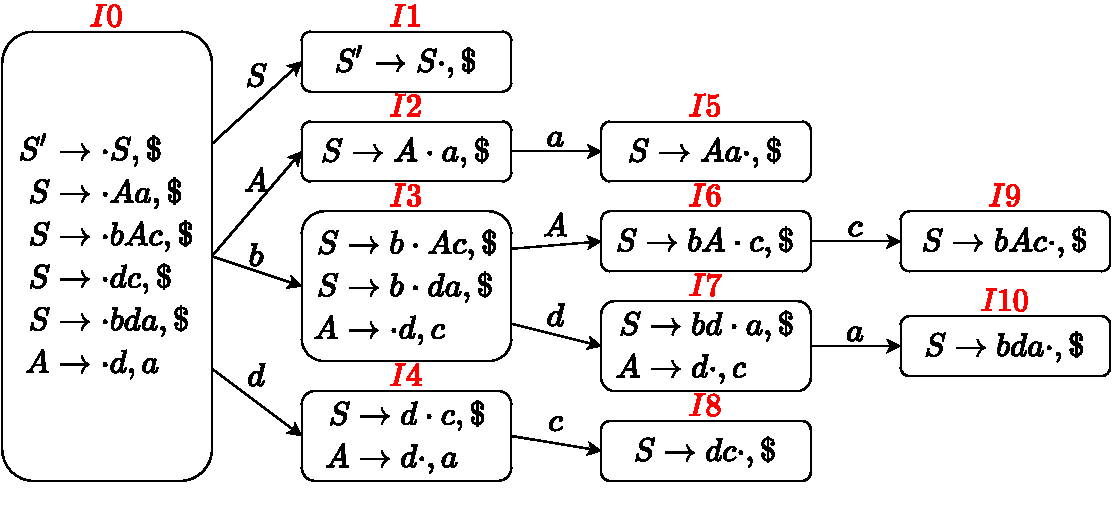
\includegraphics[width=\linewidth]{fig/T07-1.pdf}
\end{figure}
由上图知,没有相同核心(core)的状态,因此不需要合并,从而LALR分析表不冲突,该文法是LALR(1)文法。

又有$FOLLOW(A)=\{a,c\}$,考虑图中的状态$I4$,当输入符号为$c$时,$c\in FOLLOW(A)$,既有移进$S\to d\cdot c$,又有归约$S\to d\cdot$,因此SLR分析表有冲突,该文法不是SLR(1)文法。
\end{answer}

\begin{question}
证明下列文法
\[\begin{aligned}
S &\to Aa \mid bAc \mid Bc \mid bBa\\
A &\to d\\
B &\to d
\end{aligned}\]
是LR(1)文法但不是LALR(1)文法.
\end{question}
\begin{answer}
构造增广文法,得到状态$I0$。
\begin{figure}[H]
\centering
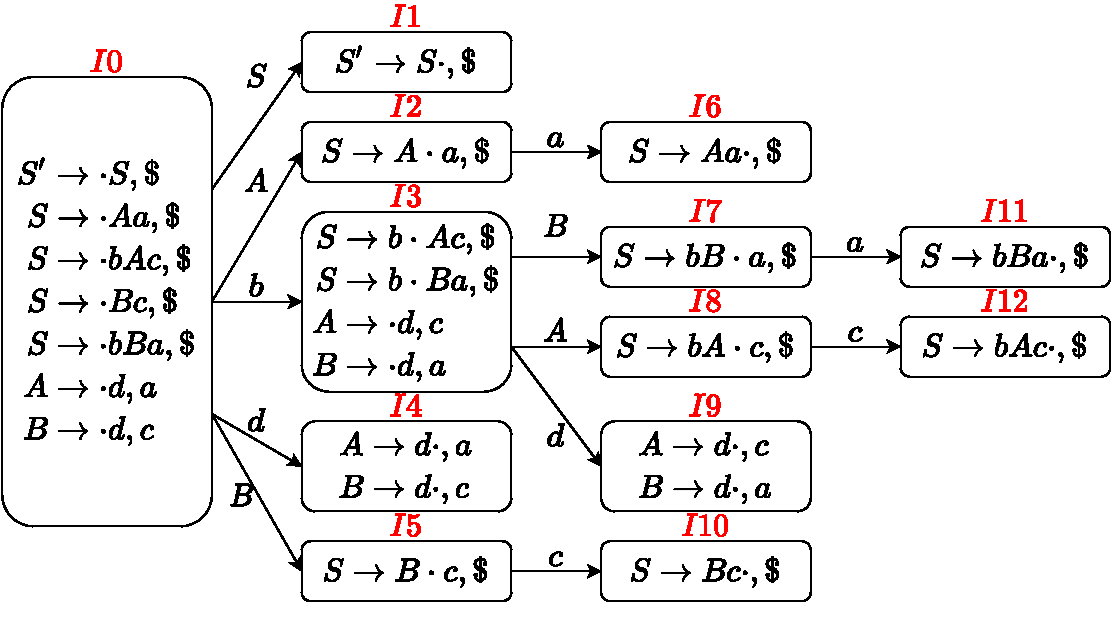
\includegraphics[width=\linewidth]{fig/T07-2.pdf}
\end{figure}
由上面的DFA知LR分析表没有冲突,因此该文法是LR(1)文法。

但如果将图中相同核心的状态$I4$和$I9$合并,会有
\[\begin{aligned}
A &\to d\cdot,a/c\\
B &\to d\cdot,a/c
\end{aligned}\]
即出现了归约-归约冲突,因此该文法不是LALR(1)文法。
\end{answer}

\end{document}